% !TeX root =  main.tex

\section{Statistical Studies}

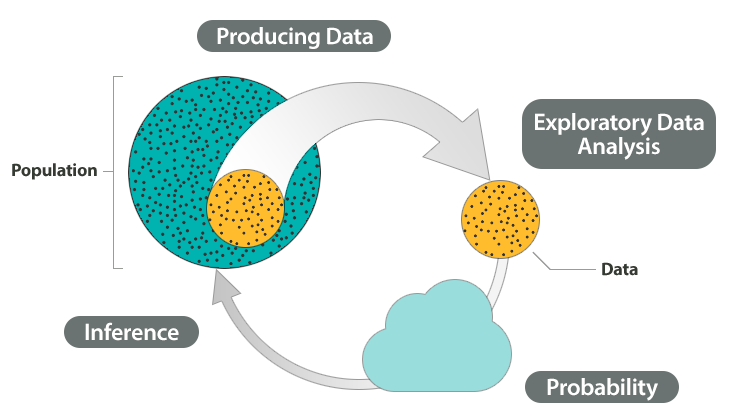
\includegraphics[scale=0.4]{Figures/Big-Picture.png}

\hypertarget{basic-statistical-concepts-14}{%
\subsection{Basic statistical concepts}\label{basic-statistical-concepts-14}}

\begin{itemize}
\item
  \textbf{Data} consists of information from observation, counts,
  measurements, responses or experiments.
\item
  A \textbf{population} is the collection of all objects that are of
  interest.
\item
  A \textbf{parameter} is a number that is a property of the population.
\item
  A \textbf{sample} is a subset of a population.
\item
  A \textbf{statistic} is a number, such as a percentage, that
  represents a property of a sample.
\item In statistics, a \textbf{variable} is a characteristic, or attribute
of interest that we gather about individuals or objects.
\item
  \textbf{Categorical variables} (or qualitative variables) represent
  attributes, labels or nonnumerical entries, such as names, and
  colors.
\item
  \textbf{Quantitative variables} represent numerical measurements or
  counts, such as weights and number of students in each class.
\end{itemize}

\begin{example}
  Identify the population, parameter, sample, and statistic in the following study: \textit{To learn the   percentage of students go to school by public transportation, 500
  students at a college were surveyed. 50\% say they go to school by
  public transportation}
\end{example}
\vspace*{2\baselineskip}

\begin{example}
  Identify the type variables.\\
\begin{enumerate*}
  \item Age
  \item Hair color
  \item GPA
  \item temperature
  \item Education attainment
\end{enumerate*}
\end{example}


\begin{exercise}
Identify the population, sample, the variable of study, the type of the
variable, the population parameter and the sample statistics.

\emph{An administrator wishes to estimate the passing rate of a certain
course. She takes a random sample of 50 students and obtains their
letter grades of that course. Among the 50 students, 32 students earned
a grade C or better.}
\end{exercise}
\vspace*{3\baselineskip}

\hypertarget{types-of-statistical-studies}{%
\subsection{Types of statistical
studies}\label{types-of-statistical-studies}}

  A statistical study can usually be categorized as an
  \textbf{observational study} or an \textbf{experiment} by the mean of
  study.

  \begin{itemize}
  \item
    An observational study observes individuals and measures variables
    of interest. The main purpose of an observational study is to
    describe a group of individuals or to investigate an association
    between two variables.
  \item
    An experiment intentionally manipulates one variable in an attempt
    to cause an effect on another variable. The primary goal of an
    experiment is to provide evidence for a cause-and-effect
    relationship between two variables.
  \end{itemize}

\begin{example}
  Which type of study will answer the question best.

  \begin{enumerate}[itemsep=2\baselineskip]
  \item
    What proportion of all college students in the United States have
    taken classes at a community college?
  \item
    Does use of computer-aided instruction in college math classes
    improve test scores?
  \end{enumerate}
\end{example}

\begin{exercise}
  Identify the type of statistical study:
  \begin{enumerate}[itemsep=2\baselineskip]
  \item
    \emph{A study took random sample of adults and asked them about their
    bedtime habits. The data showed that people who drank a cup of tea
    before bedtime were more likely to go to sleep earlier than those who didn't drink tea.}
  \item
    \emph{Another study took a group of adults and randomly divided them into two groups. One group was told to drink tea every night for a week, while the other group was told not to drink tea that week.
    Researchers then compared when each group fell asleep.}
  \end{enumerate}
\end{exercise}
\vspace*{-2\baselineskip}

\hypertarget{questions-about-population-12}{%
\subsection{Questions about population}\label{questions-about-population-12}}

\begin{longtable}[]{@{}
  >{\raggedright\arraybackslash}p{(\columnwidth - 2\tabcolsep) * \real{0.5000}}
  >{\raggedright\arraybackslash}p{(\columnwidth - 2\tabcolsep) * \real{0.5000}}@{}}
\toprule()
\begin{minipage}[b]{\linewidth}\raggedright
\textbf{Type of Research Question}
\end{minipage} & \begin{minipage}[b]{\linewidth}\raggedright
\textbf{Examples}
\end{minipage} \\
\midrule()
\endhead
\textbf{Make an estimate about the population} (often an estimate about
an \emph{average} value or a \emph{proportion} with a given
characteristic) & What is the \emph{average} number of hours that
community college students work each week? What \emph{proportion} of all
U.S. college students are enrolled at a community college? \\
\textbf{Test a claim about the population} (often a claim about an
\emph{average} value or a \emph{proportion} with a given characteristic)
& Is the \emph{average} course load for a community college student
greater than 12 units? Do the \emph{majority} of community college
students qualify for federal student loans? \\
\textbf{Compare two populations} (often a comparison of population
averages or proportions with a given characteristic) & In community
colleges, do female students have a \emph{higher} GPA than male
students? Are college athletes \emph{more} likely than non-athletes to
receive academic advising? \\
\textbf{Investigate a correlation} between two variables in the
population & Is there a \emph{correlation} between the number of hours high school students spend each week on Facebook and their GPA? Is
academic counseling \emph{associated} with quicker completion of a
college degree? \\
\bottomrule()
\end{longtable}

\begin{exercise}
  Give an example of a research question that involves
  \begin{enumerate}
    \item 
     estimating a characteristic about all students at QCC.
     \item testing a claim of a characteristic about all students at QCC.
     \item investigating a correlation between two variables about all students at QCC.
  \end{enumerate}
\end{exercise}

\hypertarget{question-on-cause-and-effect}{%
\subsection{Question on
cause-and-effect}\label{question-on-cause-and-effect}}

A research question that focuses on a cause-and-effect relationship is common in disciplines that use experiments, such as medicine or psychology.

  \begin{itemize}
  \item
    Does cell phone usage increase the risk of developing a brain tumor?
  \item
    Does drinking red wine lower the risk of a heart attack?
  \end{itemize}

In a study of a relationship between two variables, one variable is
the \textbf{explanatory variable}, and the other is the
\textbf{response variable}.

\begin{example}
  Determine if the question is a cause-and-effect question? What are the
  explanatory and response variables?
  
  \begin{enumerate}[parsep=3\baselineskip]
  \item
    Does use of computer-aided instruction in college math classes improve
    test scores?
  \item
    Does tutoring correlate with improved performance on exams?
  \end{enumerate}
\end{example}
\vspace*{-2\baselineskip}

\begin{exercise}
  A researcher studies the medical records of 500 randomly selected
  patients. Based on the information in the records, he divides the
  patients into two groups: those given the recommendation to take an
  aspirin every day and those with no such recommendation. He reports
  the percentage of each group that developed heart disease.

  Determine whether the study supports the conclusion that taking
  aspirin lowers the risk of heart attacks.
\end{exercise}
\vspace*{3\baselineskip}

\begin{exercise}
  Does higher education attainment lead to higher salary?
\begin{enumerate}[itemsep=2\baselineskip]
\item
  Determine if the question is a cause-and-effect question?
\item
  What are the explanatory and response variables?
\item
  If a student want to study this question, what type of statistical
  study can be used? What kind of conclusion can be drawn?
\end{enumerate}
\end{exercise}



\hypertarget{sampling-plans}{%
\subsection{Sampling plans}\label{sampling-plans}}

To make accurate inference, the sample must be representative of the
population.

\begin{itemize}
\item
  A \textbf{sampling plan} describes exactly how we will choose the
  sample.
\item
  A sampling plan is \textbf{biased} if it systematically favors certain
  outcomes.
\item
  In \textbf{random Sampling}, every individual or object has an equal
  chance of being selected.
\end{itemize}
\vspace*{-\baselineskip}

\hypertarget{methods-of-random-sampling-12}{%
\subsection{Methods of random sampling}\label{methods-of-random-sampling-12}}

\begin{itemize}
\item
  \textbf{Simple random sample}: groups of the same size are randomly
  selected. Table of random numbers, calculator and computer programs are often
  used to generate random numbers.
\item
  \textbf{Stratified random sample}: The population is first split into
  homogeneous groups. Then a same proportion or a same number of subjects from each group are selected randomly.

  \centerline{
    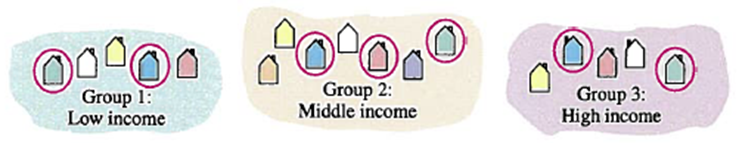
\includegraphics[scale=0.5]{Figures/Stratified-Random-Sample.png}
  }
\item
  \textbf{Cluster sample}: The population is first split into groups. Then some groups are selected randomly.

  \centerline{
    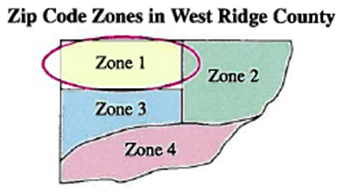
\includegraphics[scale=0.5]{Figures/Cluster-Sample.png}
  }
\item
  \textbf{Systematic sample}: First, a starting number is chosen randomly. Then take every \(n\)-th piece of the data.
  
  \centerline{
    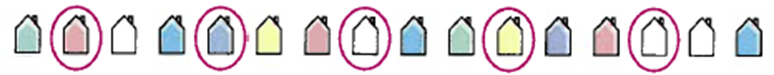
\includegraphics[scale=0.5]{Figures/Systematic-Sample.png}
  }
\end{itemize}

\begin{exercise}
Classify each of the sampling procedures below.

\begin{enumerate}[itemsep=2\baselineskip]
  \item 
  A high school educational researcher interviews 50 high school female teachers and 50 high school male teachers.
  \item The names of 25 employees being chosen out of a hat from a company of 250 employees.
  \item A researcher starts surveying every 10th customer at a local coffee shop starting at a random time between 8 am and 9 am.
  \item A student interviews classmates in his algebra class to determine how many pairs of jeans a student owns, on the average.
\end{enumerate}
\end{exercise}


\hypertarget{bad-sampling}{%
\subsection{Bad sampling}\label{bad-sampling}}

\textbf{Biased sampling}
  \begin{itemize}
  \item
    Online polls. These are examples of a voluntary response sample.
  \item
    Mall surveys. These are an example of a convenience sample.
  \end{itemize}

\textbf{Undercoverage}
  \begin{itemize}
  \item
    It occurs when some groups in the population are left out of the
    process of choosing a sample. For example, random survey math
    students to estimate the average GPA or a college.
  \end{itemize}

\begin{example}
  Suppose that you want to estimate the proportion of students at your
  college that use the library.
  
  Which sampling plan will produce the most reliable results?
  
  \begin{enumerate}[parsep=0pt]
  \item
    Select 100 students at random from students in the library.
  \item
    Select 200 students at random from students who use the Tutoring
    Center.
  \item
    Select 300 students who have checked out a book from the library.
  \item
    Select 50 students at random from the college.
  \end{enumerate}
\end{example}

\begin{exercise}
  Identify the flaw(s) in the study
  
  \textit{Students at an elementary school are given a questionnaire that they are
  asked to return after their parents have completed it. One of the
  questions asked is, ``Do you find that your work schedule makes it
  difficult for you to spend time with your kids after school?'' Of the
  parents who replied, 85\% said ``no''. Based on these results, the
  school officials conclude that a great majority of the parents have no
  difficulty spending time with their kids after school.}
\end{exercise}
\vspace*{2\baselineskip}

\hypertarget{elements-of-experimental-design-12}{%
\subsection{Elements of experimental design}\label{elements-of-experimental-design-12}}

To establish a cause-and-effect relationship, we want to make sure
  that the explanatory variable is the only thing that impacts the
  response variable. We therefore want to get rid of all other factors
  that might affect the response. These factors are called \textbf{confounding variables}.

\begin{itemize}
\item \textbf{Control} reduces the effects of confounding variables. Three control strategies are \textbf{control groups}, \textbf{placebos}, and \textbf{blinding}.

  \begin{itemize}
  \item
    A \textbf{control group} is a baseline group that receives no
    treatment or a neutral treatment.
  \item
    A neutral treatment that has no ``real" effect on the dependent
    variable is called a \textbf{placebo}, and a participant's positive response to a placebo is called the \textbf{placebo effect}.
  \item
    \textbf{Blinding} is the practice of not telling participants
    whether they are receiving a placebo. \textbf{Double-blinding} is the practice of not telling both the participants and the
    researchers which group receiving a treatment or a placebo.
  \end{itemize}

\item
  \textbf{Randomization} ensures that this estimate is statistically
  valid.
  \begin{itemize}
  \item
    With random assignment, we can be fairly confident that any
    differences we observe in the response of treatment groups is due to the explanatory variable.
  \end{itemize}

\item
  \textbf{Replication} reduces variability in experimental results and increases their significance.

  Although randomization helps to insure that treatment groups are as similar as possible, the results of a single experiment, applied to a small number of objects or subjects, should not be accepted without question.

  Any good experiment should be reproducible, and in particular, replication should yield similar results.
\end{itemize}

\begin{example}
  In the study of the relation between a type
  fertilizer and tomato size, the amount of sunshine will be a
  confounding variable. It contributes to the growth of tomato.
\end{example}
\vspace*{2\baselineskip}

\begin{exercise}
  \textit{A company tested their new golf ball by having 20 professional golfers
  each hit 100 shots with the company's new ball and 100 shots with the golfer's current ball (in a random order). The labels were removed, so the golfers didn't know which balls were which. The golfers, on average, hit their shots significantly farther with the new ball.\\  
  The company cites this study in an advertisement claiming that this new
  ball will help all golfers hit farther shots.}
  
  Is the company's claim appropriate? Why?
\end{exercise}
\vspace*{2\baselineskip}

\begin{exercise}
  \textit{Over the years it has been said that coffee is bad for you. When looking at the studies that have shown that coffee is linked to poor health, you will see that people who tend to drink coffee don't sleep much, tend to smoke, don't eat healthy, and tend to not exercise.} 
  
  Can you say that the coffee is the reason for the poor health or are there any confounding variables?
\end{exercise}
\vspace*{5\baselineskip}

\subsection{Lab 1 - Introduction to Excel}

\begin{exercise}
  In the follow figure, highlight the cell C3, the array A1:B2, and the icon for inserting function.

  \centerline{
    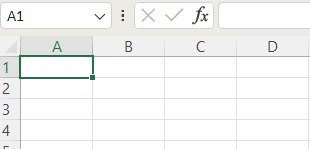
\includegraphics[scale=0.8]{Figures/Excel-CellLocator-Function.png}
  }
\end{exercise}

\begin{exercise}
  Describe how to use the Excel autofill function to generate a sequential array.
\end{exercise}
\vspace*{3\baselineskip}

\begin{exercise}
  Write down two Excel functions that can be used to generate random numbers and describe the difference.
\end{exercise}
\vspace*{3\baselineskip}

\begin{exercise}
  Describe approach on how to use the paste special option to convert a row array into a column array.
\end{exercise}
% \vspace*{3\baselineskip}

% \begin{exercise}
%   Describe how to use autofill to add a number in the cell B1 to each number in the array A1:A10.
% \end{exercise}